\documentclass{article}

\usepackage{graphicx}
\usepackage{tikz}
\usepackage{tikzsymbols}
\usetikzlibrary{calc,patterns,shapes.geometric}
\pagestyle{empty}
\usepackage[margin=0pt]{geometry}
\geometry{papersize={14in,12in}}

\def\centerarc[#1](#2)(#3:#4:#5){\draw[#1] ($(#2)+({#5*cos(#3)},{#5*sin(#3)})$) arc (#3:#4:#5);}

\begin{document}
	\begin{figure}
		\centering
		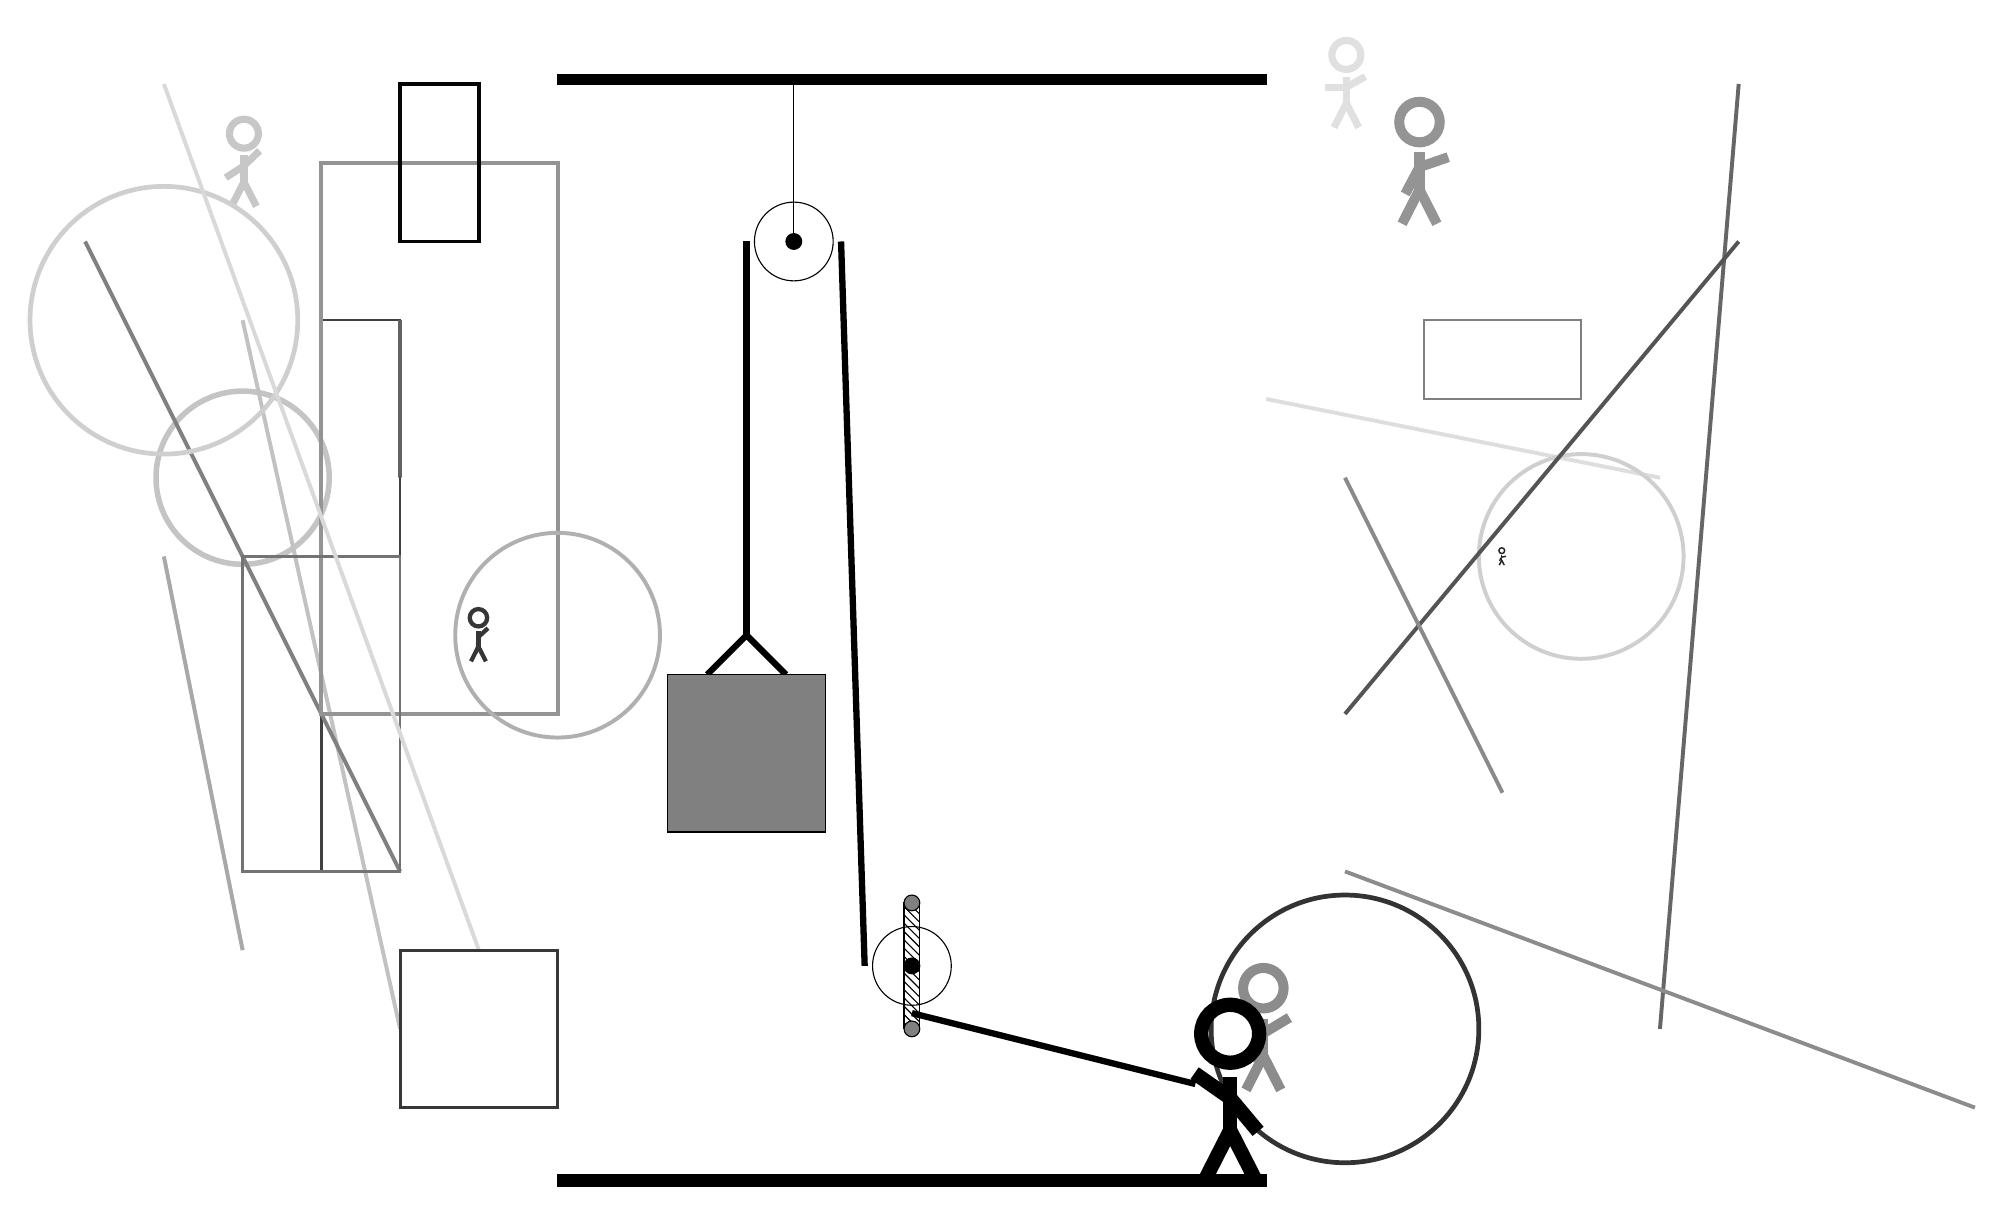
\begin{tikzpicture}
			%%%%% START %%%%%
			
			\draw[fill=black] (-2, 14) rectangle (7, 14.125);
			
			\draw (1, 12) circle (0.5);
			\draw[fill=black] (1, 12) circle (0.1);
			\draw (1, 14) -- (1, 12);
			
			\draw [line width=0.7mm, color=black!23](-6, 9) circle (1.1);
			
			\draw[line width=0.5mm, color=black!60](12, 2) -- (13, 14);
			\draw[line width=0.5mm, color=black!13](7, 10) -- (12, 9);
			\node[line width=0.4mm, color=black!22] at (-6, 13) {\Strichmaxerl[5][33][44]};
			\draw[line width=0.3mm, color=black!75] (-4, 4) rectangle (-5, 11);
			\draw[line width=0.2mm, color=black!50] (9, 10) rectangle (11, 11);
			
			\draw[line width=0.5mm, color=black!62] (-4, 11) rectangle (-4, 9);
			\draw[line width=0.5mm, color=black!24](-6, 11) -- (-4, 2);
			\draw [line width=0.5mm, color=black!19](11, 8) circle (1.3);
			\draw[line width=0.5mm, color=black!50](-4, 4) -- (-8, 12);
			
			\draw [line width=0.6mm, color=black!80](8, 2) circle (1.7);
			\draw[line width=0.5mm, color=black!45](8, 4) -- (16, 1);
			\draw[line width=0.5mm, color=black!42] (-2, 6) rectangle (-5, 13);
			\draw[line width=0.5mm, color=black!98] (-3, 12) rectangle (-4, 14);
			\draw [line width=0.6mm, color=black!19](-7, 11) circle (1.7);
			\node[line width=0.7mm, color=black!45] at (7, 2) {\Strichmaxerl[7][77][31]};
			\node[line width=0.3mm, color=black!79] at (-3, 7) {\Strichmaxerl[3][87][43]};
			\draw [line width=0.5mm, color=black!31](-2, 7) circle (1.3);
			\node[line width=0.2mm, color=black!12] at (8, 14) {\Strichmaxerl[5][0][29]};
			\draw[line width=0.3mm, color=black!55] (-4, 8) rectangle (-6, 4);
			\node[line width=0.5mm, color=black!42] at (9, 13) {\Strichmaxerl[7][62][19]};
			
			\draw[line width=0.5mm, color=black!15](-7, 14) -- (-3, 3);
			
			\draw[line width=0.4mm, color=black!78] (-4, 3) rectangle (-2, 1);
			\draw [line width=0.7mm, color=black!66](-6, 9) circle (0.0);
			\draw [line width=0.2mm, color=black!51](-4, 13) circle (0.0);
			\draw[line width=0.5mm, color=black!67](8, 6) -- (13, 12);
			\draw[line width=0.5mm, color=black!34](-6, 3) -- (-7, 8);
			\draw[line width=0.5mm, color=black!46](10, 5) -- (8, 9);
			\node[line width=0.3mm, color=black!87] at (10, 8) {\Strichmaxerl[1][59][10]};
			
			
			\draw[fill=white](2.5, 2.8) circle (0.5);
			\draw[fill=black] (2.5, 2.8) circle (0.1);
			\draw[pattern=north west lines, pattern color=black] (2.4, 3.6) rectangle (2.6, 2.0);
			\draw[fill=black!50] (2.5, 3.6) circle (0.1);
			\draw[fill=black!50] (2.5, 2.0) circle (0.1);
			
			\draw[line width=0.8mm] (-0.1, 6.5) -- (0.4, 7.0) -- (0.9, 6.5);
			\draw[fill=black!50] (-0.6, 6.5) rectangle (1.4, 4.5);
			
			\draw[line width=0.8mm] (0.4, 12) -- (0.4, 7.0);
			\centerarc[line width=0.8mm](1, 12)(0:180:0.6);
			\draw[line width=0.8mm](1.6, 12) -- (1.9, 2.8);
			\centerarc[line width=0.8mm](2.5, 2.8)(180:270:0.6);
			\draw[line width=0.8mm](2.5, 2.2) -- (6.1, 1.3);
			
			\node at (6.5, 1.2) {\Strichmaxerl[10][-35][-50]};
			
			\draw[fill=black] (-2, 0) rectangle (7, 0.15);
			
			%%%%% END %%%%%
		\end{tikzpicture}
	\end{figure}	
\end{document}